\documentclass{article}
\usepackage[utf8]{inputenc}
\usepackage{amsmath}
\usepackage{amssymb}
\usepackage{mathtools}
\usepackage{graphicx}
\usepackage{mcode}
\usepackage[export]{adjustbox}
\usepackage{caption}
\captionsetup[figure]{labelformat=empty}

\graphicspath{{Images/}}

\setlength{\oddsidemargin}{0in}
\setlength{\textwidth}{6.5in}
\setlength{\topmargin}{-.55in}
\setlength{\textheight}{9in}
\pagestyle{empty}


\title{Scientific Computation Midterm 1}
\author{Michael Nameika}
\date{October 2022}

\begin{document}

\maketitle

\section*{Exercise 1}

Consider the eigenvalue BVP
\[u''(x) = \lambda u(x), \:\:\: u(0) = u(1) = 0\]
which has eigenvalues $\lambda_n = -(n\pi)^2$, $n = 1, 2, \dots$.
\begin{enumerate}
    \item[(a)] Using finite differences, devise a numerical algorithm for computing these eigenvalues. Implement it in Matlab and discuss how good is the approximation in terms of the mesh size $h$. Plot the eigenfunctions for the first few eigenvalues.
    \newline
    
    Using the 3-point stencil to approximate the second derivative:
    \[\frac{u(x + h) - 2u(x) + u(x - h)}{h^2} = u''(x) + \mathcal{O}(h^2)\]
    we can write the eigenvalue problem as the following linear system:
    \[AU = h^2\lambda U\]
    where $A$ is an $(n+1) \times (n+1)$ matrix and $U \in \mathbb{R}^n$ are defined by the following:
    \begin{align*}
        A &= \begin{bmatrix}
            -2 & 1 & & & \\
            1 & -2 & 1 & & \\
            & \ddots & \ddots & \ddots & \\
            &  & 1 & -2 & 1 \\
            & & & 1 & -2 \\
        \end{bmatrix}, \:\:\:\:  U = \begin{bmatrix}
            u(t_1) \\
            u(t_2) \\
            \vdots \\
            u(t_{n+1}) \\
        \end{bmatrix} \\
    \end{align*}
    Then from the linear system above, it is clear to see that the eigenvalues of $A$ are $h^2\lambda$. That is, if we compute the eigenvalues of $A$ and divide by $h^2$, we will recover the (approximate) eigenvalues of the eigenvalue problem. Implementing this into matlab and running the code for $h = 10,20,\dots, 100$ we find the following error plot when compared with the first four true eigenvalues:
    \begin{center}
        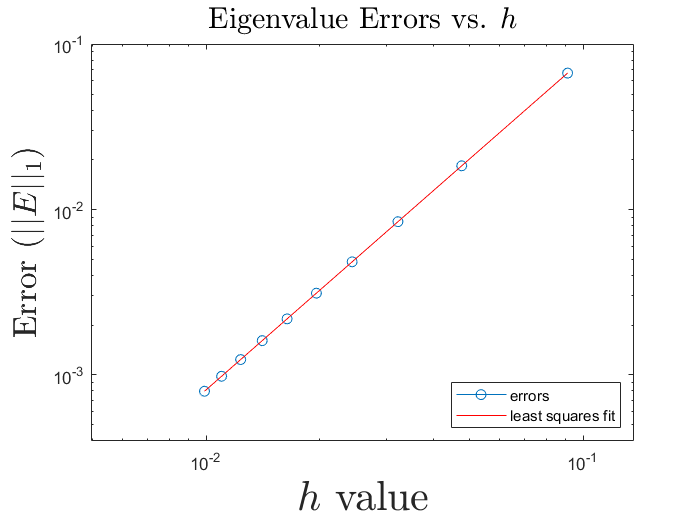
\includegraphics[scale = 0.45]{eigenvalueEerror.png}
        \newline
        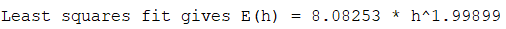
\includegraphics[]{errorOrder.PNG}
    \end{center}
    As we can see, this method is very close to second order accurate, which we should expect from a second order method. Now, let us inspect the first few eigenfunctions:
    \newline
    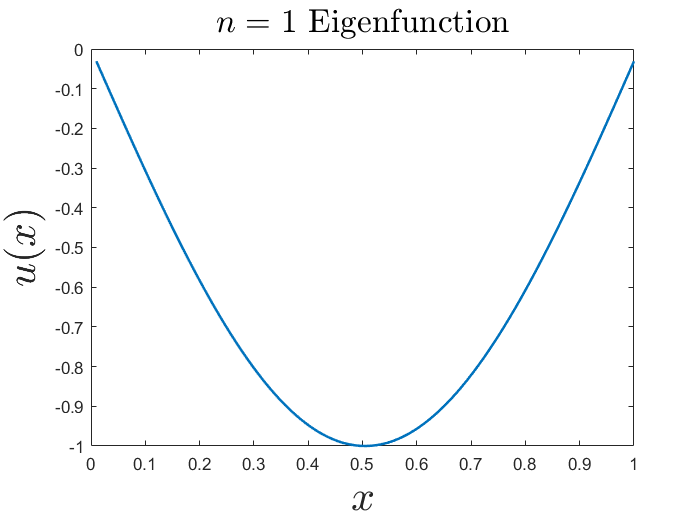
\includegraphics[scale = 0.4]{1aeig1.png}
    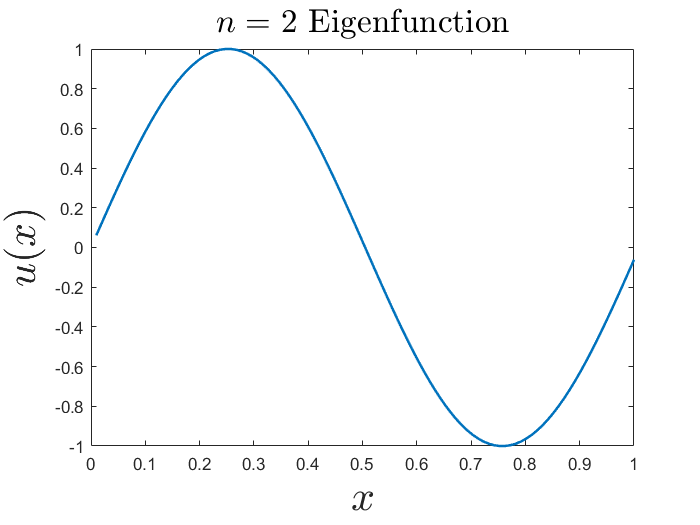
\includegraphics[scale = 0.4]{1aeig2.png}
    \newline
    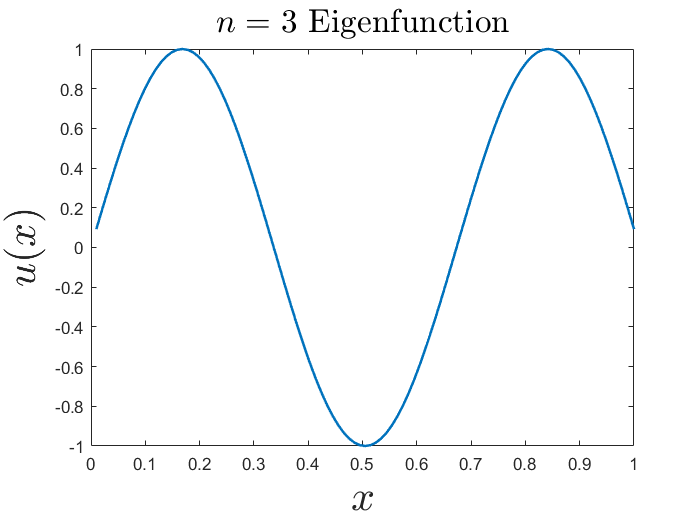
\includegraphics[scale = 0.4]{1aeig3.png}
    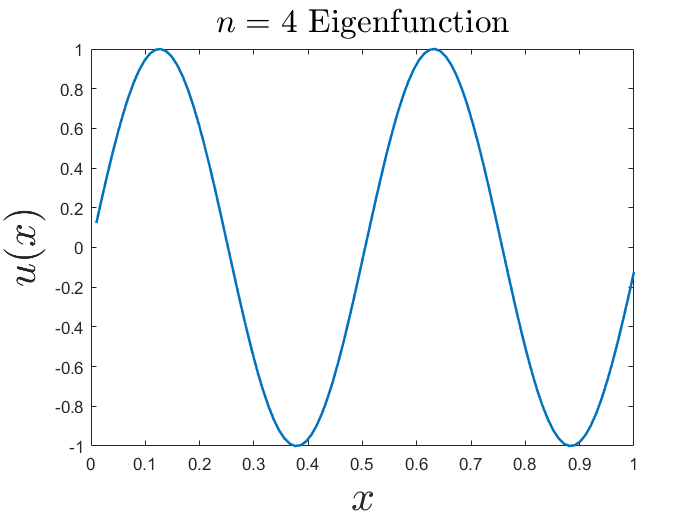
\includegraphics[scale = 0.4]{1aeig4.png}
    \newline
    Which is what we would expect since the eigenvalue problem has solutions of the form $u(x) = C\sin{(n\pi x)}$.
  
    
    See attached code for details. 
    
    \item[(b)] Adapt your algorithm and code from (a) to the eigenvalue BVP
    \[u''(x) = \lambda u(x), \:\: u(0) = 0, \:\: u'(1) + u(1) = 0.\]
    for which the eigenvalues cannot be computed explicitly. Again, plot the first few eigenfunctions.
    \newline\newline
    Doing the problem analytically, we find that the eigenvalues satisfy the following transcendental equation:
    \[\tan{(\sqrt{\lambda})} + \sqrt{\lambda} = 0\]
    
    From the above conditions, we have $u_{m+1} + u'_{m+1} = 0$. Using the approximation $u_{m+1}' \approx (u_{m+1} - u_{m})/h$, we have
    \begin{align*}
        u_{m+1} + u_{m+1}/h - u_m/h &= 0 \\
        (1 + h)u_{m+1} - u_m = 0 \\
    \end{align*}
    Then changing the last row of the matrix $A$ to include this condition, and multiplying the right hand side by an identity matrix with the last row consisting of only zeros to correct for the final boundary condition, and finding the eigenvalues, we find the following first few eigenvalues compared to the eigenvalues computed numerically:
    
    \begin{figure}[!h]
        \begin{center}
            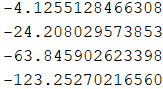
\includegraphics[]{eigapprox1b.PNG}
            \caption{Eigenvalues calculated from finite differences}
        \end{center}
    \end{figure}
    \begin{figure}[!h]
        \begin{center}
            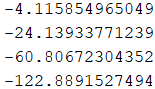
\includegraphics[]{trueeig1b.PNG}
            \caption{Eigenvalues calculated numerically from transcendental equation}
        \end{center}
    \end{figure}
    \begin{figure}[!h]
        \begin{center}
            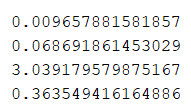
\includegraphics[]{err1b.PNG}
            \caption{Absolute error of eigenvalues}
        \end{center}
    \end{figure}
    
    Now, let's inspect the first few eigenfunctions:
    
    \begin{center}
        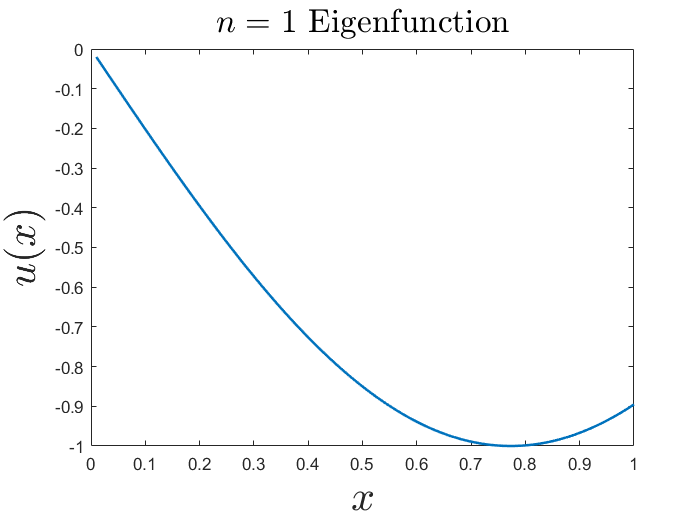
\includegraphics[scale = 0.4]{1beig1.png}
        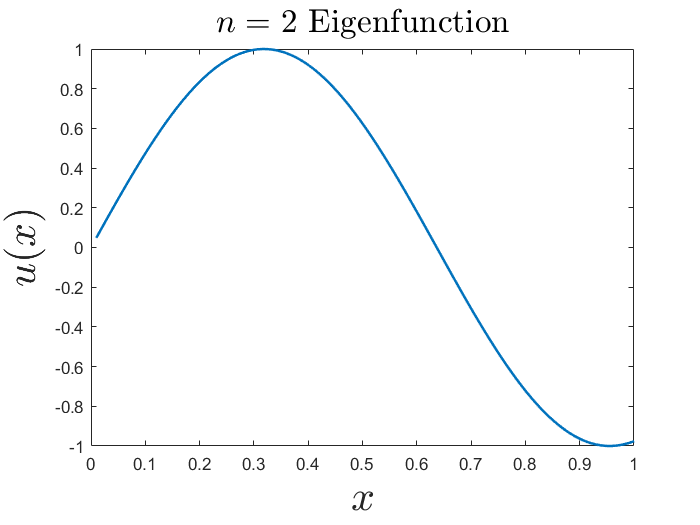
\includegraphics[scale = 0.4]{1beig2.png}
        \newline
        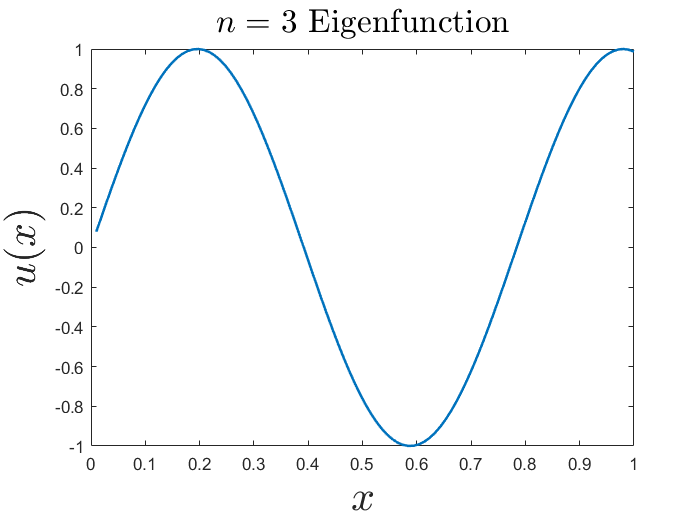
\includegraphics[scale = 0.4]{1beig3.png}
        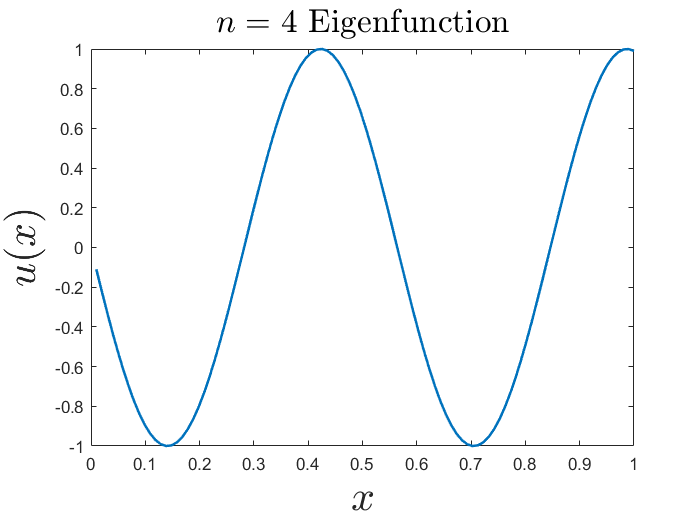
\includegraphics[scale = 0.4]{1beig4.png}
        \newline
    \end{center}
    
    \item[(c)] Consider the eigenvalue problem for the 2-dim Laplacian
    \[\Delta u = \lambda u\]
    in the unit square $[0,1] \times [0,1]$ with Dirichlet boundary conditions using the 5-point Laplacian and explain how well are the eigenvalues $\lambda_{m,n} = -(m^2 + n^2)\pi^2$ approximated. Plot eigenfunctions for the first few eigenvalues.
    \newline\newline
    Using the given MATLAB code poisson.m to create the $A$ matrix for the 5-point Laplacian, and finding the first four eigenvalues for $m=5,10,15,20$, we find the following:
    \begin{center}
        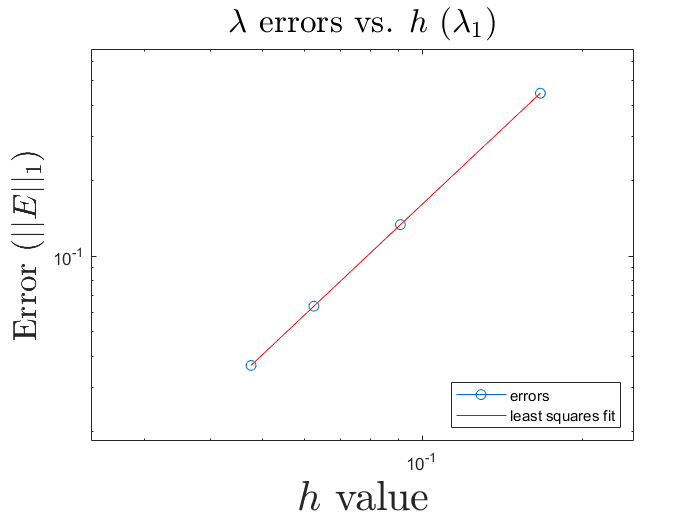
\includegraphics[scale = 0.4]{laplaceLam1.png}
        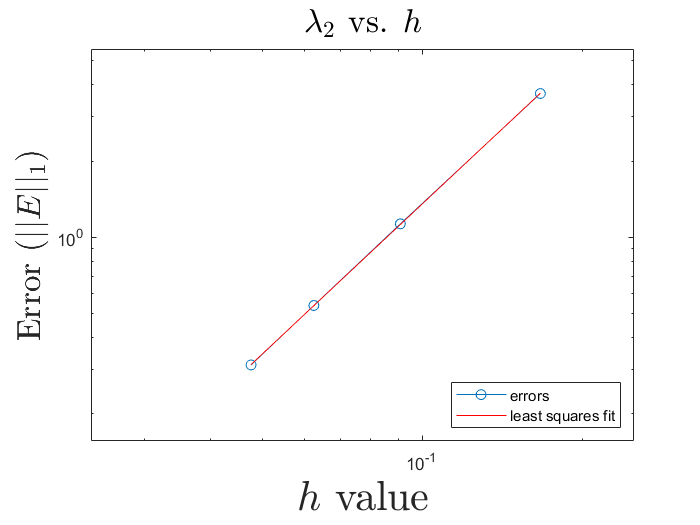
\includegraphics[scale = 0.4]{laplaceLam2.png}
        \newline
        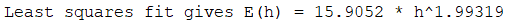
\includegraphics[scale = 0.6]{lam1err.PNG} \:\:\:\:
        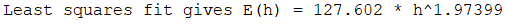
\includegraphics[scale = 0.6]{lam2err.PNG}
        \newline
        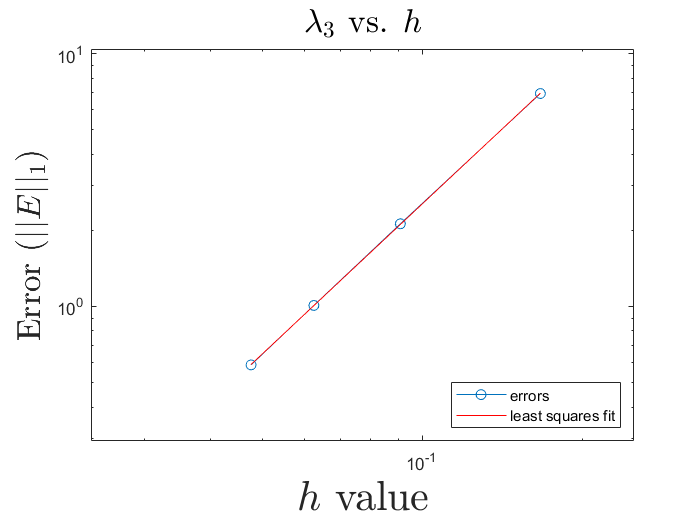
\includegraphics[scale = 0.4]{laplaceLam3.png}
        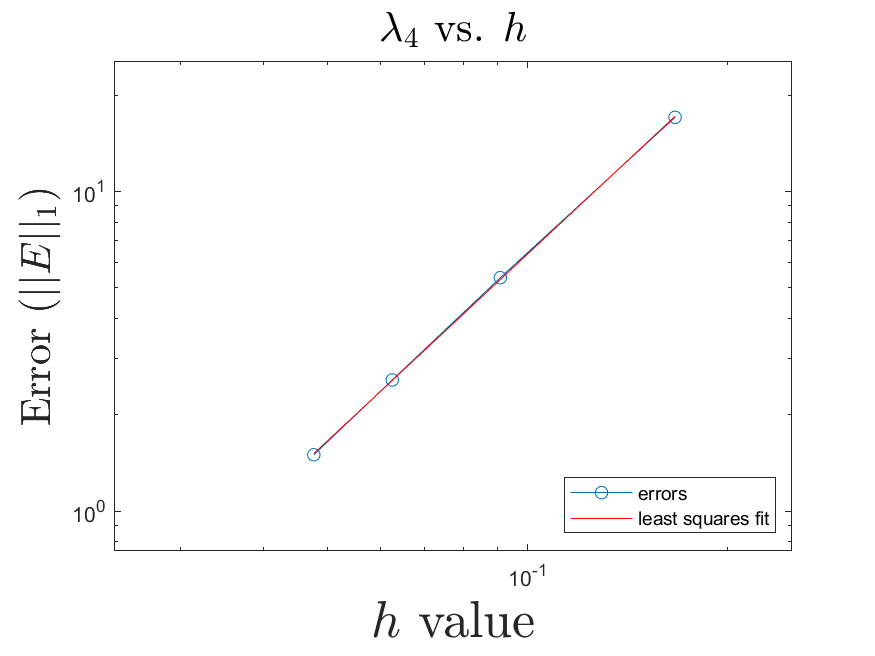
\includegraphics[scale = 0.5]{laplaceLam4.png}
        \newline
        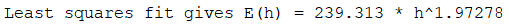
\includegraphics[scale = 0.6]{lam3err.PNG} \:\:\:\:
        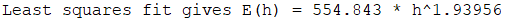
\includegraphics[scale = 0.6]{lam4err.PNG}
    \end{center}
    So we can see that this second order method is approximately second order accurate for the first four eigenvalues. Now, let us inspect the first four eigenfunctions:
    \begin{center}
        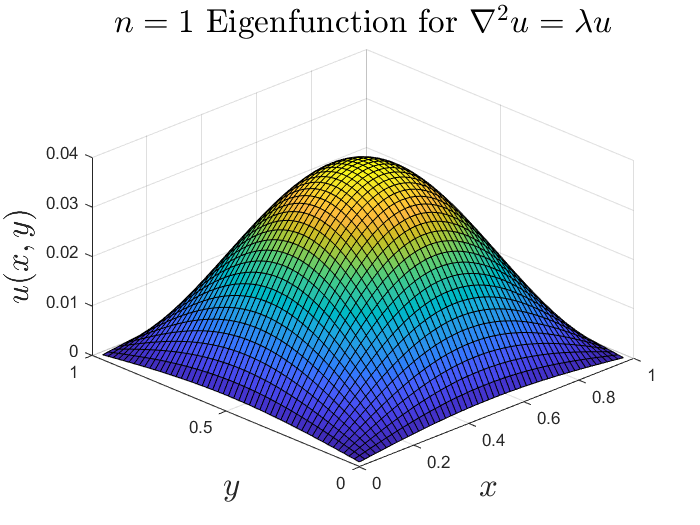
\includegraphics[scale = 0.4]{n1eig.png}
        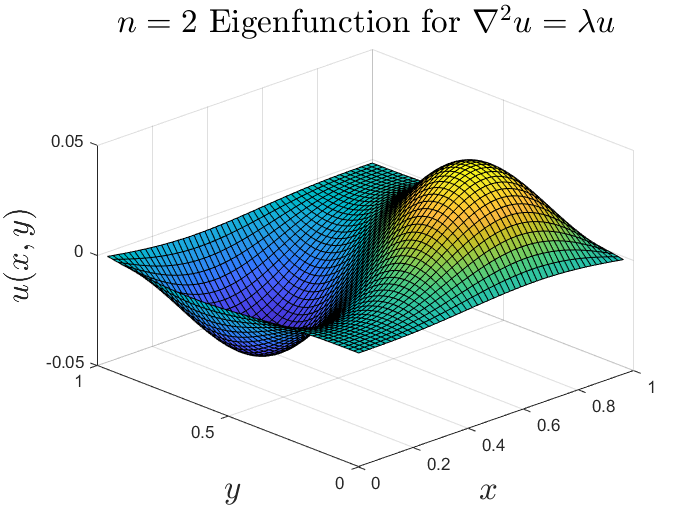
\includegraphics[scale = 0.4]{n2eig.png}
        \newline
        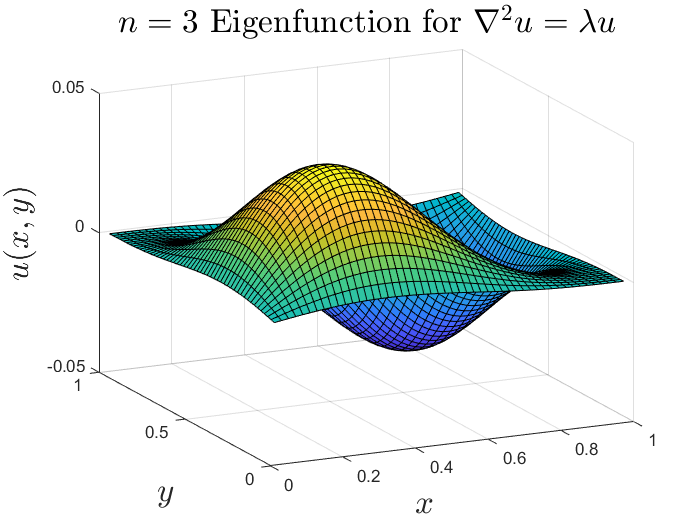
\includegraphics[scale = 0.4]{n3eig.png}
        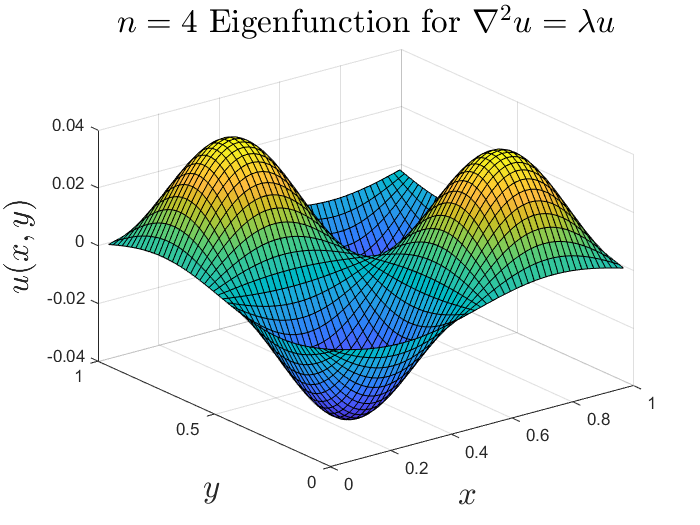
\includegraphics[scale = 0.4]{n4eig.png}
    \end{center}
\end{enumerate}


\section*{Exercise 2}
An implicit $r$-step LMM of the form
\[U^{n+r} = U^{n+r-2} + h\sum_{j=0}^r\beta_jf(t_{n+j},U^{n+j}), \: \beta_r \neq 0\]
is known as (implicit) Milne method.
\begin{enumerate}
    \item[(a)] Derive the 2-step third-order accurate Milne method, starting from the relation
    \[u(t_{n+2}) = u(t_n) + \int_{t_n}^{t_{n+2}}f(s,u(s))ds\]
    and following the procedure described in exercise 5.10 (b) in Leveque book. 
    \newline\newline
    To begin, let us interpolate $f(s,u(s))$ for the points $s = t_n, t_{n+1}, t_{n+2}$ and let $t_n = -h$, $t_{n+1} = 0$, $t_{n+2} = h$ for ease of computation (the coefficients for the interpolating polynomial will be independent of $s$, so we may make this assumption). Let's proceed by Lagrange interpolation:
    \begin{align*}
        P(s) &= f(U^n)\frac{(s-t_{n+1})(s-t_{n+2})}{(t_n - t_{n+1})(t_n - t _{n+2})} + f(U^{n+1})\frac{(s-t_n)(s-t_{n+2})}{(t_{n+1} - t_{n})(t_{n+1} - t_{n+2})} + f(U^{n+2})\frac{(s-t_n)(s - t_{n+1})}{(t_{n+2} - t_n)(t_{n + 2} - t_{n+1})} \\
        &= \frac{1}{2h^2}f(U^n)(s^2-sh) - \frac{1}{h^2}f(U^{n+1})(s^2-h^2) + \frac{1}{2h^2}f(U_{n+2})(s^2 + sh) \\
    \end{align*}
    integrating, we find
    \begin{align*}
        \int_{t_n}^{t_{n+2}}P(s) &= \int_{t_n}^{t_{n+2}}\frac{1}{2h^2}f(U^n)(s^2-sh) - \frac{1}{h^2}f(U^{n+1})(s^2-h^2) + \frac{1}{2h^2}f(U_{n+2})(s^2 + sh) ds \\
        &= \frac{1}{h^2}\left[\frac{1}{2}f(U^n)\left(\frac{s^3}{3}- \frac{s^2}{2}h\right) - f(U^{n+1})\left(\frac{s^3}{3} - sh^2\right) + \frac{1}{2}f(U^{n+2})\left(\frac{s^3}{3} + \frac{s^2}{2}h\right)\right]\bigg|_{-h}^h \\
        &= \frac{h}{3}\left[f(U^n) + 4f(U^{n+1}) + f(U^{n+2})\right] \\
    \end{align*}
    Putting it together, we have for Milne's method,
    \[U^{n+2} = U^{n} + \frac{h}{3}\left[f(U^n) + 4f(U^{n+1}) + f(U^{n+2})\right]\]
    
    \item[(b)] Use the implicit Milne's method to solve numerically the ODE
    \[u'(t) = 2(t + 1), \:\:\: u(1) = 3\]
    Implementing Milne's method in MATLAB, we find the following plots for the approximate solution plotted with the exact solution. See attached code for additional details.
\end{enumerate}
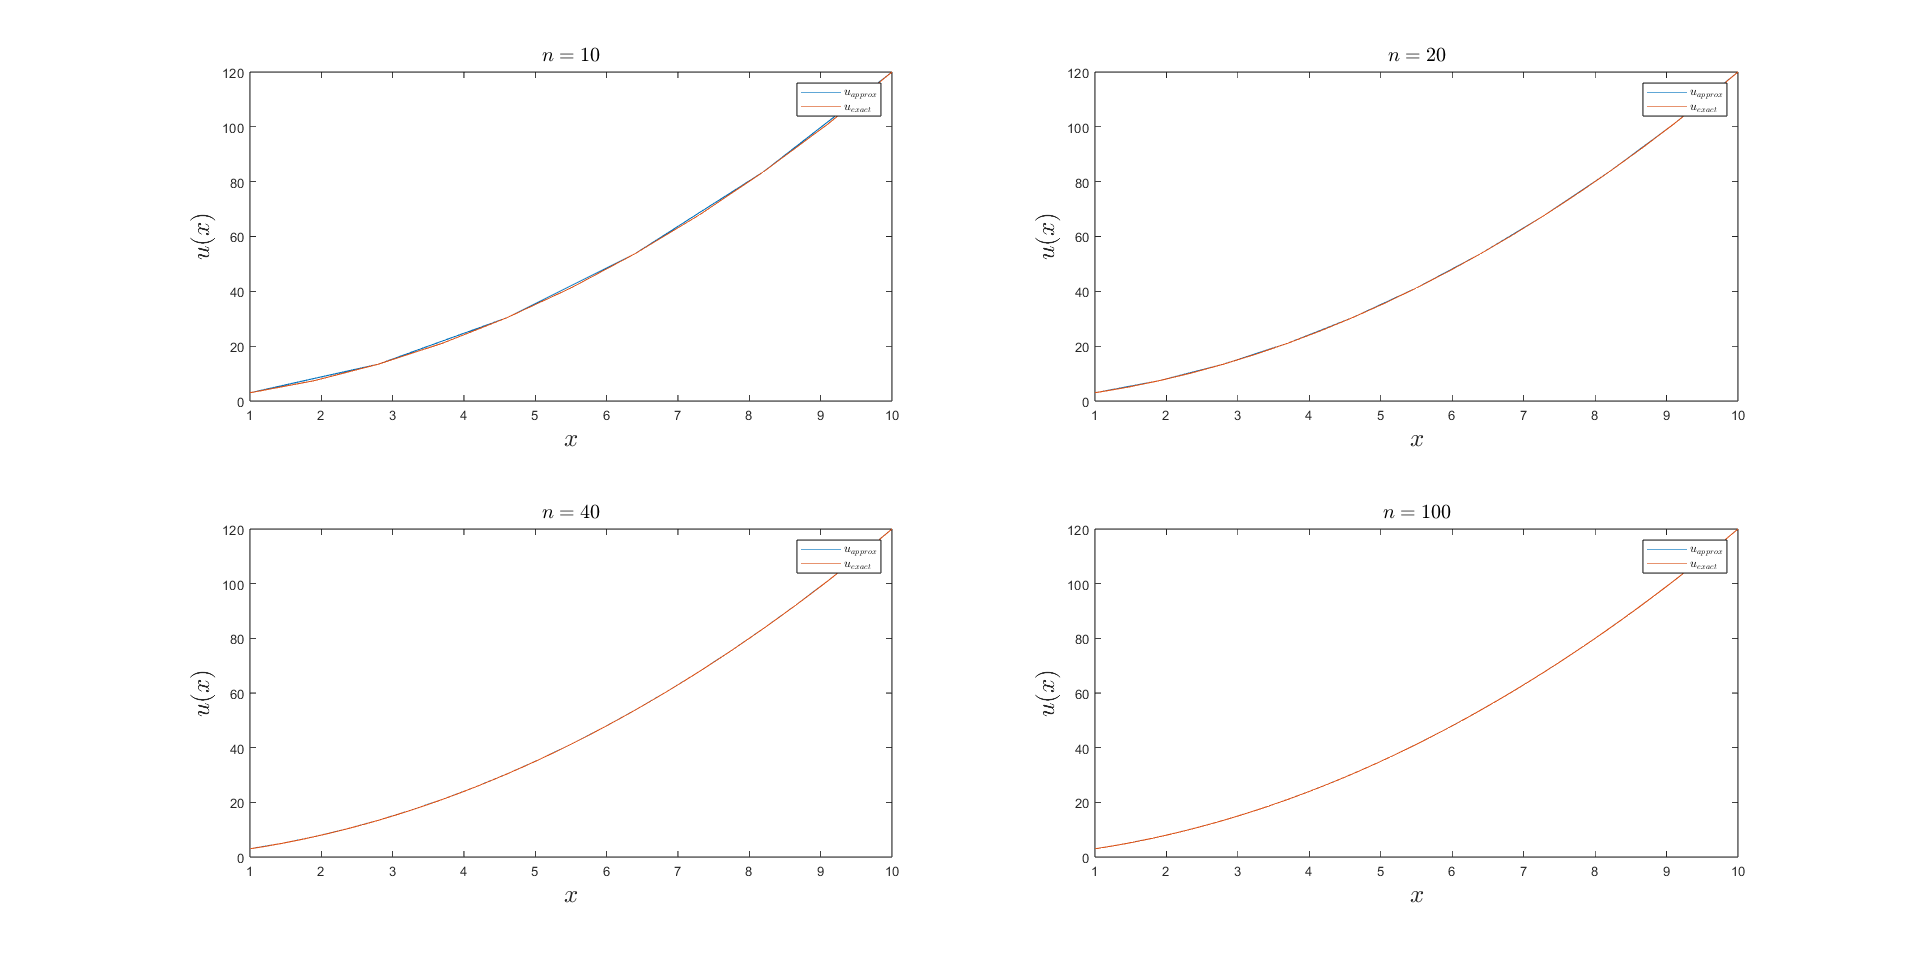
\includegraphics[scale = 0.35]{milneplots.png}
\newline

\section*{Exercise 3}
Consider the implicit Runge Kutta method
\begin{align*}
    U^* = U^n + h/2f(t_n + h/2, U^*)& \\
    U^{n+1} = U^n + hf(t_n + h/2, U^*)& \\
\end{align*}
\begin{enumerate}
    \item[(a)] Determine the order of accuracy of this method
    \newline\newline
    Let us determine the order of accuracy of this method by finding the order of accuracy for $u'(t) = \lambda u$. For this differential equation, we have $f(t,u(t)) = \lambda u(t)$. Then 
    \begin{align*}
        &U^* = U^n + \frac{h}{2}\lambda U^* \\
        &U^*\left(1 - \frac{h\lambda}{2}\right) = U^n \\
        &U^* = \frac{1}{1 - \frac{h\lambda}{2}} U^n \\
    \end{align*}
    Then notice
    \begin{align*}
        U^{n+1} &= U^n + h\lambda U^* \\
        &= U^n + \frac{h\lambda}{1 - \frac{h\lambda}{2}} U^n \\
    \end{align*}
    Now, recall the Taylor expansion for $1/(1-x)$:
    \[\frac{1}{1-x} = \sum_{n=0}^{\infty} x^n\]
    Then for $x = h/2$, we get
    \[\frac{1}{1 - \frac{h}{2}} = 1 + \left(\frac{h\lambda}{2}\right) + \left(\frac{h\lambda}{2}\right)^2 + \mathcal{O}(h^3)\]
    Substituting this expansion into the equation we found for $U^{n+1}$, we find
    \begin{align*}
        U^{n+1} &= U^n + h\lambda U^n + \frac{h^2 \lambda^2}{2} U^n + \frac{h^3\lambda^3}{4}U^n + \mathcal{O}(h^4) \\
        &= U^n\left(1 + h\lambda + \frac{h^2\lambda^2}{2}\right) + \mathcal{O}(h^3) \\
        &= U^ne^{h\lambda} + \mathcal{O}(h^3) \\
    \end{align*}
    Notice that we recover the Taylor expansion for $e^{h\lambda}$ up to second order term. Thus, the order of accuracy of this implicit Runge Kutta method is second order accurate.
    
    
    \item[(b)] Determine the absolute stability region. Is it A-stable? Is it L-stable?
    \newline\newline
    Notice from part (a) before we do the Taylor expansion, we have the relation
    \[U^{n+1} = \left(1 + \frac{h\lambda}{1 - \frac{h\lambda}{2}}\right)U^n\]
    Making the substitution $z = h\lambda$, we have
    \begin{align*}
        U^{n+1} &= \left(1 + \frac{2z}{2-z}\right)U^n \\
        &= R(z)U^n \\
    \end{align*}
    where $R(z) = 1 + 2z/(2-z)$. Notice we may rewrite $R(z)$ as the following:
    \[R(z) = \frac{2 + z}{2 - z}\]
    Then our region of absolute stability is satisfied whenever
    \[\frac{|2 + z|}{|2 - z|} \leq 1\]
    Notice that this inequality has no restrictions for $\text{Im}(z)$, but we require $\text{Re}(z) \leq 0$. That is, our region of absolute stability is $\text{Re}(z) \leq 0$.
    \newline
    
    Clearly, this method is A-stable (the region of absolute stability is exactly the definition of A-stability!). However, the method is not L-stable. Notice the following:
    \begin{align*}
        \lim_{z \to \infty} |R(z)| &= \lim_{z \to \infty} \frac{|2 + z|}{|2 - z|} \\
        &= \lim_{z \to \infty} \frac{|2/z + 1|}{|2/z - 1|} \\
        &= 1 \neq 0 \\
    \end{align*}
    So this method is not L-stable.
    
    \item[(c)] Use this method to solve the initial value problem $u'(t) = 2(t + 1), \: u(1) = 3$.
    \newline\newline
    Notice for this problem that this implicit Runge Kutta method becomes explicit. Implementing it into matlab, we find the following error plot for multiple values of $h$:
    \begin{center}
        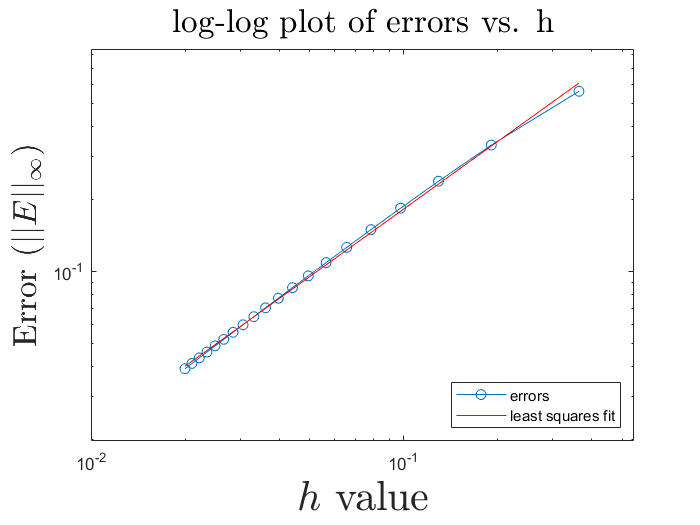
\includegraphics[scale = 0.5]{3cerr.png}
        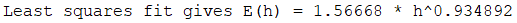
\includegraphics[scale = 0.7]{3cleastsquares.PNG}
    \end{center}
    And observe the following plots of the approximate solution plotted against the exact solution:
    \begin{center}
        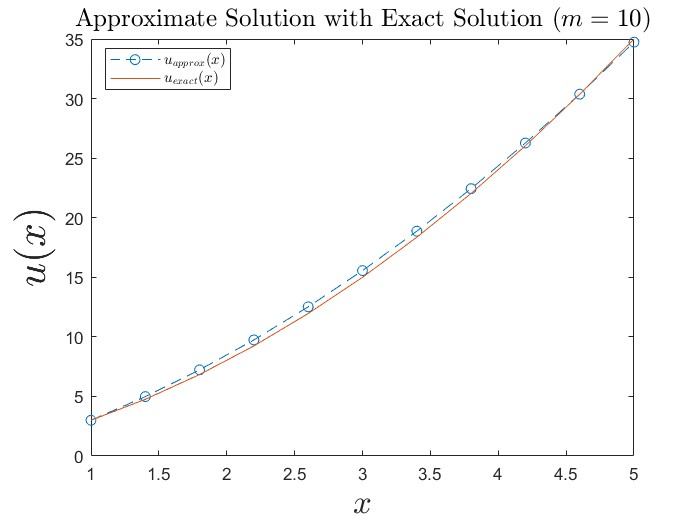
\includegraphics[scale = 0.4]{3cm10.png}
        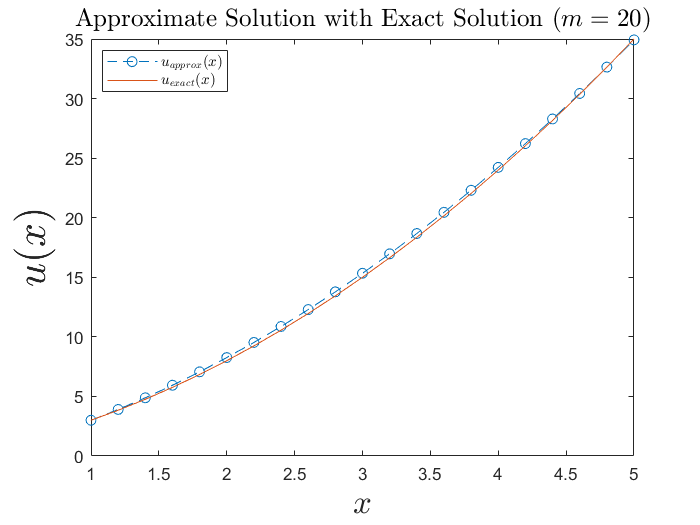
\includegraphics[scale = 0.4]{3cm20.png}
        \newline
        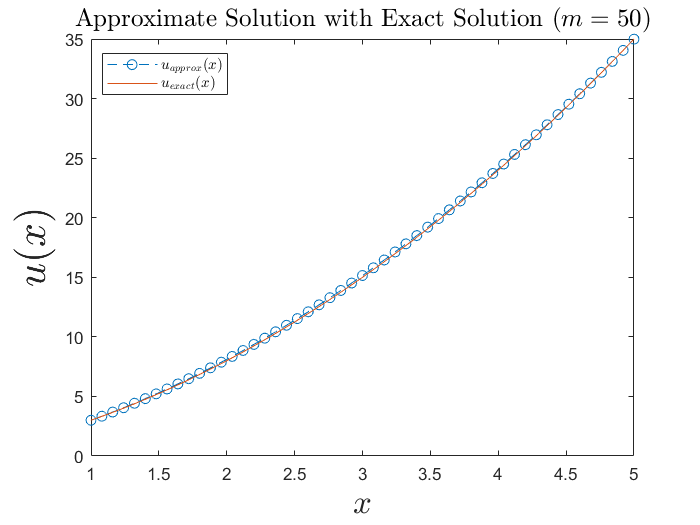
\includegraphics[scale = 0.4]{3cm50.png}
        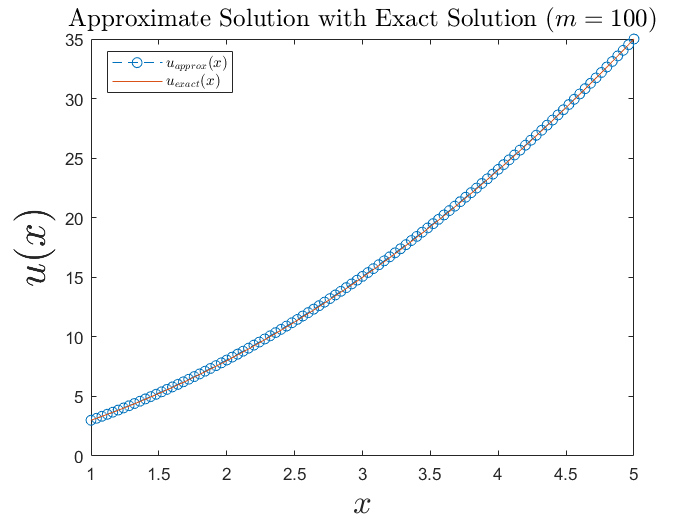
\includegraphics[scale = 0.4]{3cm100.png}
    \end{center}
    
\end{enumerate}

\section*{Exercise 4}
(a) Consider the second order problem
\[u''(x) = xu(x), \:\:\:\: x \geq 0\]
which has a unique solution $u(x)$ with $u(\infty) = 0$. The challenge is to numerically find this solution. You may approach it as a boundary value problem or as an initial value problem. 
\newline\newline
I will approach this problem as an initial value problem using the built in ode45 solver in MATLAB. Turning the problem into a system of first order differential equations, we may write the problem as
\begin{align*}
    v_1' &= v_2 \\
    v_2' &= xv_1 \\
\end{align*}
For this problem I will be looking at the interval $[0,10]$. Since $u(\infty) = 0$, we may assume that the value of $u(x)$ and $u'(x)$ will get small as $x$ gets large. Then using ode45, with the interval \mcode{tRange = linspace(10,0,1000)}. We start from 10 and go to 0 so as to apply the initial conditions at $t = 10$. Calling on ode45 like \mcode{[t, x] = ode45(@F, tRange, [1e-4 1e-4])} (see attached F.m code), we find
\begin{center}
    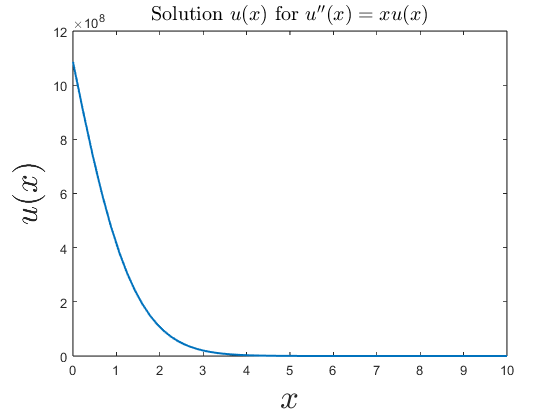
\includegraphics[scale = 0.6]{prob4plot1.png}
\end{center}
doing some research, I found that the Airy function of the first kind has a value of approximately 0.355 at $t = 0$. Then normalizing this graph so that the value at $x = 0$ is approximately 0.355, we find the following:
\begin{center}
    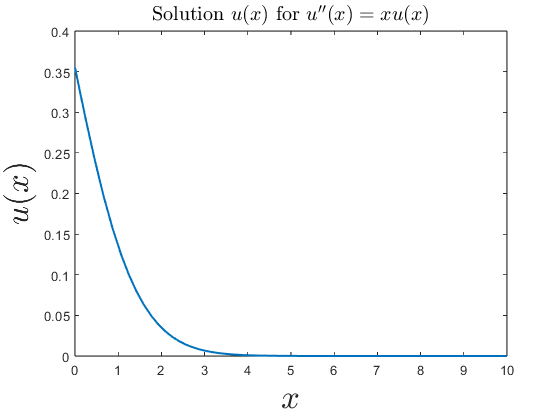
\includegraphics[scale = 0.6]{prob4plot2.png}
\end{center}
which roughly has the form of the of the Airy function of the first kind. And just for fun, let's inspect the plot of our approximate solution and the built in Airy function in MATLAB:
\begin{center}
    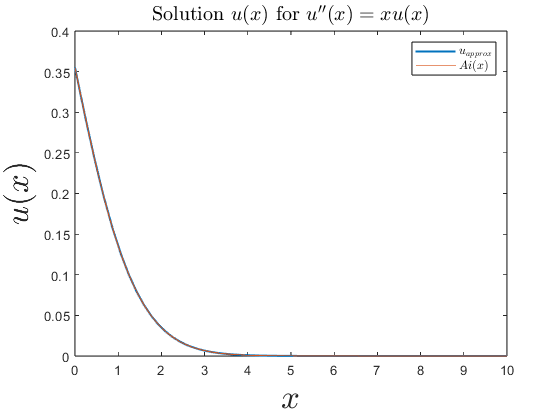
\includegraphics[scale = 0.5]{approxvsai.png}
\end{center}




\end{document}
